\setchapterpreamble[u]{\margintoc}
\chapter{Պատահական մեծություններ}
\labch{random_variables}

\emergencystretch 2em

\section{Ֆորմալ սահմանումը}

Նախորդ թեմայի վերջին խնդիրը լուծելիս ունեինք երկու անհայտ մեծություններ՝ ավտոբուսի գալու ժամանակն ու մեր գալու ժամանակը, որոնց արժեքը հայտնի չէր (ընդունում էին պատահական արժեքներ), սակայն գիտեինք, թե որոնք էին դրանց հավանական արժեքները, այնպես որ դրանք նշանակեցինք տառերով ու լուծեցինք խնդիրը։ Նմանատիպ մեծությունները, որոնց արժեքը չգիտենք, բայց կարող ենք \textit{հաշվել,} թե ինչ հավանականությամբ են ընդունում այս կամ այն արժեքը, \marginnote{անգլերեն՝ {\it random variables}} կոչվում են \textit{պատահական մեծություններ։}

\question{Փողոցում մոտենում եք պատահական անցորդի ու հարց\-նում նրա հասակը։ Մոտավորապես ո՞ր միջակայքի արժեքներն են ավելի շատ հավանական, որո՞նք՝ ավելի քիչ։}

Եթե փորձենք ավելի ճշգրիտ ձևակերպում տալ, կարող ենք փողոցում քայլող բոլոր հնարավոր մարդկանց բազմությունը համարել մեր $\Omega$-ն, և ասել, որ պատահական ընտրված ցանկացած մարդու համապատասխա\-նեց\-րել ենք ինչ-որ մի թիվ՝ նրա հասակը։ Կամ որ նույնն է՝ ստեղծել ենք $X$ ֆունկցիա, որը վերցնում է $\omega$ մարդուն ու վերադարձնում նրա հասակը՝ $X(\omega)$։ 

\begin{example}\label{die_game}
Խաղում ենք հետևյալ խաղը․ նետում ենք զառը, պարզ թիվ ընկնելու դեպքում շահում ենք $100$ դրամ, բաղադրյալ թվի դեպքում՝ կորցնում $100$, հակառակ դեպքում՝ լինում է ոչ-ոքի։ Այս դեպքում մեր վերջնական շահումը/կորուստը կլինի պատահական մեծություն։ 

Եթե նշանակենք այն $X$-ով, ապա $X$-ը կընդունի երեք արժեք՝
\[ X  =
\begin{cases}
100 & \text{եթե } \omega \in \{2, 3, 5\} \\
-100 & \text{եթե } \omega \in \{4, 6\} \\
0 & \text{եթե } \omega \in \{1\}
\end{cases}
\]
Կարո՞ղ եք հաշվել հավանականությունը, որ $X=100$։
\end{example}

Առհասարակ՝ ցանկացած բան, որի արժեքը կախված է ինչ-որ  պատահական փորձի արդյունքից, հանդիսանում է պատահական մեծություն։

\begin{example}\label{rv_examples}
Դիտարկենք հետևյալ պատահական փորձերը․

\begin{enumerate}
\item Նետում ենք երկու զառ։ Դրանց ելքերի գումարը պատահական մեծություն է։

\item Երկու թիմ խաղում են ֆուտբոլ։ Նրանց խփած գոլերի թիվը, ինչպես նաև հաշվի տարբերությունը պատահական մեծու\-թյուններ են։ 

\item Զանգահարում ենք պատահական հեռախոսահամարով և հարցնում, թե քանի երեխա կա ընտանիքում․ սա նույնպես պատա\-հական մեծություն է։

\item Ընդհանուր քանի հաղորդագրություն կստանաք վաղը՝ պատա\-հական մեծություն է։

\item Երկու ավտոբուս պատահական պահերի անցնում են կանգառով։ Դրանցից յուրաքանչյուրի գալու պահը, ինչպես նաև այդ երկու պահերի տարբերությունը պատահական մեծություններ են։

\item Որքան կլինեն «{\rm Apple}»-ի արժեթղթերը հաջորդ շաբաթ՝ պատահական մեծություն է։

\item $xy$-հարթության վրա պատահական նշված կետի երկու կոոր\-դի\-նատները, նաև այդ կետի հեռավորությունը, ասենք, $(5, 3)$ կետից՝ պատահական մեծություններ են։
\end{enumerate}
\end{example}

\question{Որո՞նք են նշված պատահական մեծություններից յուրա\-քան\-չյուրի հնարավոր արժեքները։}

\begin{example}
Նետում ենք երկու զառ։ Այն, թե
\begin{itemize}
    \item ո՞վ է նետել զառերը
    \item ի՞նչ գույն ունի երկինքը
    \item ինչո՞ւ է աղմկում գետը
    \item ի՞նչ թիվ է ընկել երրորդ զառը
\end{itemize}
պատահական մեծություններ \textit{չեն,} քանի որ դրանք \textit{կախված չեն} կատարված փորձի արդյունքից․ եթե նույնիսկ իմանայինք, թե ինչ են ընկել զառերը, այս հարցերին չէինք կարող պատասխանել։
\end{example}

Այսպիսով, ինտուիտիվ դժվար չէ հասկանալ, թե այս կամ այն խնդրում ինչն է պատահական մեծություն։ \marginnote{այսինքն՝ չափել, թե որքան է հավանա\-կան, որ $X$-ի արժեքը կլինի այս կամ այն բազմությունից (թե չէ ամբողջ տեսու\-թյունն անիմաստ կդառնար)}
Եթե այնուամենայնիվ փորձենք ավելի ճշգրիտ սահմանել, կասենք, որ ցանկացած այնպիսի $X$, որի արժեքների հավանականությունը կարող ենք չափել, պատահական մեծություն է։

\warning{Առջևում սպասվում է տեսական բնույթի քննարկում։}

Իսկ հավանականությունը չափելու համար անհրաժեշտ է մեկ բան։ Որպեսզի, օրինակ, կարողանանք հաշվել, թե ինչ հավանականությամբ է $X$-ը ընդունում $1.57$ արժեքը՝ 
\[
\PP[X = 1.57]
\]
անհրաժեշտ է, որ $\PP[\quad]$-ի մեջ գրվածը լինի պատահույթ, այսինքն՝
\[
\{X = 1.57\} = \{ \text{այն $\omega$-ները, որոնց համար }X = 1.57 \} \in \F
\]
Նույն ձև բնականաբար պետք է կարողանանք չափել $\PP[X < 1.57]$, $\PP[X > 1.57]$, $\PP[X \le 1.57]$ և մնացած այլ հավանականությունները։

\question{Ունենալով $\PP[X \le 1.57]$-ը՝ կարո՞ղ եք հաշվել $\PP[X > 1.57]$-ը։}

Ուրեմն ֆորմալ կպահանջենք, որ ասենք՝ $\{X \le 1.57\}$ բազմությունը լինի պատահույթ ($=$ հնարավոր լինի չափել դրա հավանականությունը), կամ ընդհանուր դեպքում՝ ցանկացած $c$ թվի համար
\[
\{X \le c\} = \{ \text{այն $\omega$-ները, որոնց համար }X \le c \} \in \F
\]
լինի պատահույթ։ \marginnote{կարող ենք իհարկե $\le$-ի փոխարեն գրել $<$, $>$ կամ $\ge$} Ահա այս պայմանին բավարարող ցանկացած $X$ կանվանենք պատահական մեծություն։

Նշենք, որ հետագա կիրառություններում բավարար է ընդամենը համա\-րել, որ ցանկացած անհայտ, բայց խելքին մոտիկ բան պատահական մեծություն է։ 

Նկատենք նաև, որ եթե $X$-ը ինչ-որ մի պատահական մեծություն է, ապա նրա հետ գործողություններ անելիս՝
\begin{itemize}
    \item $2X$-ը
    \item $X+4$-ը
    \item $X^2$-ն
    \item $e^X$-ը
\end{itemize}
և այլն նույնպես կլինեն պատահական մեծություններ։ 

Ավելի ընդհանուր,
\begin{theorem}\label{transformed_rv}
Եթե $X$-ը պատահական մեծություն է, ապա $g(X)$-ը նույնպես պատահական մեծություն է (ցանկացած $g$ անընդհատ ֆունկցիայի համար)։
\end{theorem}



\section{Դիսկրետ պատահական մեծություններ}

Ինչպես նկատում ենք, որոշ պատահական մեծությունների հնարավոր ար\-ժեքները կարելի է ներկայացնել ցուցակի տեսքով, օրինակ՝ $\{2, 3, 4, \linebreak \dots, 12\}$ կամ $\{0, 1, 2, \dots\}$, իսկ որոշներինը՝ միջակայքերի՝ $(0, +\infty)$։

Եթե պատահական մեծության հնարավոր արժեքների բազմությունը
\begin{itemize}
    \item վերջավոր է՝ $\{x_1, x_2, \dots, x_n\}$, կամ անվերջ, բայց հաշվելի՝ $\{x_1, x_2, \dots, x_n, \dots\}$, \marginnote{այսինքն անվերջ, բայց միջակայքեր չպարունակող, օրինակ՝ $\N$-ը}ապա այն կանվանենք \textit{դիսկրետ} կամ \textit{ընդհատ}

    \item իսկ եթե այն ինչ-որ միջակայք է՝ $(a,b)$ կամ $[a, b]$ (կամ դրանց միավորում), ապա այն կանվանենք \textit{անընդհատ}
\end{itemize} 

Մասնավորապես, ցանկացած բանի քանակ ցույց տվող պատահական մեծությունները դիսկրետ են, իսկ ժամանակ կամ երկարություն ցույց տվողները՝ անընդհատ։ \hyperref[rv_examples]{{\color{OliveGreen} Օրինակ \ref*{rv_examples}}}-ի 1-4 դեպքերում պատահական մեծությունները դիսկրետ են, 5-7-ում՝ անընդհատ։

\question{$X$-ով նշանակենք զառի թվի մնացորդը $3$-ի բաժանելիս․
\begin{itemize}
    \item ի՞նչ հնարավոր արժեքներ կարող է այն ընդունել
    \item որքա՞ն է դրանցից յուրաքանչյուրի հավանականությունը
    \item որքա՞ն է հավանական, որ $X=5$
\end{itemize}}

Իհարկե, եթե որևէ անհայտ բան նշանակել ենք $X$-ով, նախ և առաջ կուզեինք պարզել, թե որքան է հավանական, որ այն կընդունի այսինչ արժեքը։ Վերցնենք ասենք՝ \hyperref[die_game]{{\color{OliveGreen} օրինակ \ref*{die_game}}}-ի խաղում մեր շահույթը ցույց տվող $X$ պատահական մեծությունը․
\[ 
X  =
\begin{cases}
100 & \text{եթե } \omega \in \{2, 3, 5\} \\
-100 & \text{եթե } \omega \in \{4, 6\} \\
0 & \text{եթե } \omega \in \{1\}
\end{cases}
\]

Որքա՞ն է հավանականությունը, որ կշահենք $100$ դրամ, այսինքն՝
\[
\PP[X = 100] =\  ? 
\]
Քանի որ $X$-ը $100$ արժեքը ընդունում է $\{2, 3, 5\}$ ելքերի դեպքում, $X=1$-ի հավանականությունը կլինի հենց այդ պատահույթի հավանականու\-թյու\-նը՝
\[
\PP[X = 100] = \PP[\{2, 3, 5\}] = \frac{3}{6} = 0.5
\]
իսկ օրինակ ոչ-ոքիի հավանականությունը՝
\[
\PP[X = 0] = \PP[\{1\}] = \PP[1] = \frac{1}{6}
\]
Հետևյալ արտահայտությունը՝
\[
\PP[X = \text{ինչ-որ թիվ}]
\]
որը վերևում հաշվեցինք, ըստ էության ֆունկցիա է, որը վերցնում է $c$ թիվն ու վերադարձնում $X$-ի՝ այդ $c$ թվին հավասար լինելու հավանականությունը՝
\[
p_X(c) = \PP[X = c]
\]
այսինքն հաշվում, թե որքան է հավանական, որ ${X=c}$։ Այդ $p_X$ ֆունկ\-ցիան կանվանենք $X$-ի \textbf{հավանականային ֆունկցիա} կամ {\bf PMF:}\marginnote{{\it probability mass function}}

\question{Ենթադրենք $X$-ը հենց զառը նետելիս ստացվող թիվն է։ Կարո՞ղ եք գրել կամ պատկերել դրա հավանականային ֆունկցիան։}

{\rm PMF}-ի շնորհիվ, օրինակ՝ եթե ունենք դրա գրաֆիկը, կարող ենք պատ\-կե\-րացում կազմել, թե ի՞նչ արժեք\-ներ է ընդունում $X$-ը, արժեքներից ո՞րը ի՞նչ հավանականությամբ, և այլն։

\question{Քանի՞ ֆիլմ եք դիտելու հաջորդ ամիս։ Պատասխանը նշա\-նա\-կենք $X$-ով և գծենք նրա {\it PMF}-ի գրաֆիկը։ Որքա՞ն է հավա\-նական, որ կդիտեք $5$-$6$ ֆիլմ։ Քանի՞ ֆիլմն է ամենահավանականը։}

\begin{figure}[b]
    \centering
    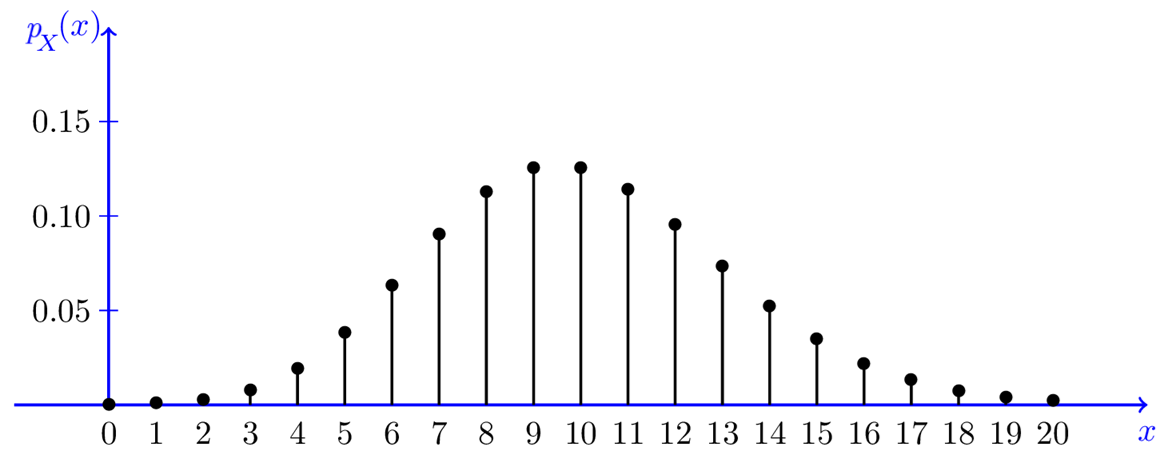
\includegraphics[width=0.8\linewidth]{chapters/chapter 9/PMF graph.png}
\end{figure}

\begin{example}
Ուսանողը գիտի հարցաշարի $15$ թեմաներից $4$-ը, ընդ որում քննության ժամանակ տրվելու է $2$ հարց։ $X$-ով նշանակենք, թե այդ երկու հարցից քանիսին կպատասխանի ուսանողը, և հաշվենք $X$-ի {\rm PMF}-ը։

Հավանականությունը, որ ուսանողը ոչ մի հարցի չի պատասխանի, նույնն է, ինչ եթե և՛ առաջին, և՛ երկրորդ հարցերը լինեն նրա չիմացած հարցերից․\marginnote[*+1]{$\Rightarrow$ պետք էր ժամանակին սովորել}
\[
\PP[X=0] = \frac{11}{15} \cdot \frac{10}{14} = \frac{11}{21} \approx 0.52
\]
իսկ որպեսզի երկուսին էլ կպատասխանի, անհրաժեշտ է, որ և՛ առաջինը, և՛ երկրորդը լինեն իր իմացածներից․
\[
\PP[X=2] = \frac{4}{15} \cdot \frac{3}{14} = \frac{6}{105} \approx 0.06
\]
Մնաց մի դեպք՝ երկու հարցից ուղիղ մեկին պատասխանելու դեպքը, որի հավանականությունը կլինի\marginnote{կարող էինք հաշվել նաև այսպես՝ \[\PP[X=1] = \frac{4}{15} \cdot \frac{11}{14} + \frac{11}{15} \cdot \frac{4}{14}\]}
\[
\PP[X=1] = 1 - \PP[X=0] - \PP[X=2] 
% = 1 - \frac{11}{21} - \frac{6}{105} 
= \frac{44}{105} \approx 0.42
\]\begin{marginfigure}[*+4]
    \centering
    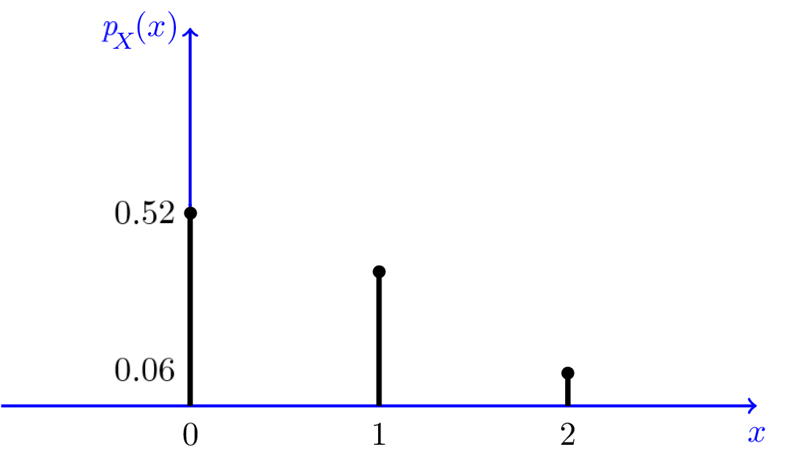
\includegraphics[width=\linewidth]{chapters/chapter 9/PMF graph exam.png}
\end{marginfigure}
Հետևաբար $X$-ի {\rm PMF}-ն է՝
\[
p_X(k) \approx \begin{cases}
    0.52 & \text{եթե } k = 0\\
    0.42 & \text{եթե } k = 1\\
    0.06 & \text{եթե } k = 2\\
    0 & \text{եթե $k$-ն այլ թիվ է}
\end{cases}
\]
որը ցանկության դեպքում կարող ենք ներկայացնել աղյուսակով՝
\begin{center}
% \begin{table}[h]
  % \centering
  % \raggedright
  \begin{tabular}{|c|c|}
    \hline
    $k$ & $\PP[X=k]$ \\
    \hline
    $0$ & $0.52$ \\
    \hline
    $1$ & $0.42$ \\
    \hline
    $2$ & $0.06$ \\
    \hline
  \end{tabular}
% \end{table}
\end{center}
\end{example}


\section{Բաշխման ֆունկցիա}

Հավանականային ֆունկցիան, իհարկե, կարևոր է իմանալ, բայց այս իրավիճակում ուսանողին հետաքրքրում է ոչ այնքան իր պատասխանած հարցերի թիվը, որքան քննության արդյունքը՝ կկտրվի՞, թե՞ ոչ։ 

Եթե օրինակ՝ անցողիկ շեմը լիներ ճիշտ պատասխանել $1$ հարցի, կտրվելու հավանականությունը կլիներ
\[
\PP[X < 1] = \PP[X = 0] \approx 0.52
\]
իսկ եթե լիներ $2$ հարց՝
\[
\PP[X < 2] = \PP[X = 0] + \PP[X = 1] \approx 0.94
\]
Գոյատևելու շանսերը կլինեին համապատասխանաբար $1-0.52=0.48$ և $1-0.94=0.06$: 

Մի ուրիշ իրավիճակում հնարավոր միավորների թիվը կարող էր լինել $1$-ից մինչև $20$՝ յուրաքանչյուր արժեքը իր հավանականությունով։ Այս դեպքում ևս, եթե ուսանողը ցանկանար հաշվել իր կտրվելու (ասենք՝ $10$ միավոր կամ ցածր հավաքելու) հավանականությունը, կգրեր
\[
\PP[X \le 10] = \PP[X = 0] + \PP[X = 1] + \dots + \PP[X = 10]
\]
իսկ քննությունը ստանալունը կլիներ $1 - \PP[X \le 10]$:

Գործնականում հաճախ է պետք գալիս առանձին-առանձին $1$, $2$, $\dots$, $k$ արժեքներն ընդունելու հավանականություններից բացի ունենալ նաև $k$-ից փոքր, մեծ, փոքր կամ հավասար լինելու հավանականությունը՝
\[
\PP[X \le k]
\]
Բայց այստեղ ևս $k$-ի տարբեր արժեքներ տեղադրելով՝ ստանում ենք տարբեր թվեր, հետևաբար գործ ունենք $k$-ից կախված ֆունկցիայի հետ։ Ուրեմն 
{\rm PMF}-ի նմանությամբ սահմանենք հետևյալ ֆունկցիան՝
\[
F_X(k) = \PP[X \le k]
\]
և անվանենք այն $X$-ի \textbf{բաշխման ֆունկցիա} կամ {\bf CDF:}\marginnote{{\it cumulative distribution function}}

\question{Ուսանողի օրինակում ինչի՞ է հավասար $X$-ի {\rm CDF}-ը։}

\begin{example}
$X$-ով նշանակենք զառը նետելիս ստացված թիվը և գտնենք դրա բաշխման ֆունկցիան։ Սկսենք $k=1$-ից՝
\[
F_X(1) = \PP[X \le 1] = \frac{1}{6}
\]
քանի որ $X$-ը $1$-ից փոքր արժեք չի կարող ընդունել։ 

Իսկ ասենք $k=2$ արժեքի դեպքում՝
\[
F_X(2) = \PP[X \le 2] = \PP[X = 1] + \PP[X = 2] = \frac{2}{6} = \frac{1}{3}
\]
Նույն կերպ $k=3$-ի համար $F_X(3) = \dfrac{3}{6}$, ապա
\[
F_X(4) = \dfrac{4}{6} \qquad F_X(5) = \dfrac{5}{6} \qquad F_X(6) = \dfrac{6}{6} = 1
\]

Իսկ ի՞նչ, եթե $F_X$-ի մեջ տեղադրենք $6$-ից մեծ թիվ, ասենք՝ $k=8$։ Կունենանք՝
\[
F_X(8) = \PP[X \le 8] = 1
\]
քանի որ $X$-ի արժեքը \textit{միշտ փոքր է} $8$-ից։ Նույն ձևով $F_X(k) = 1$ բոլոր այնպիսի $k$ թվերի համար, որոնք մեծ են $6$-ից։ 

Մյուս կողմից՝ եթե տեղադրենք $1$-ից փոքր արժեք, ասենք՝
\[
F_X(0.12) = \PP[X \le 0.12] = 0
\]
կունենանք $0$, քանի որ $X$-ը \textit{երբեք փոքր չէ} $1$-ից։ Հետևաբար $F_X(k) = 0$ բոլոր $k < 1$ թվերի համար։

Վերջապես եթե տեղադրենք ոչ ամբողջ թիվ, օրինակ՝
\[
F_X(5.5) = \PP[X \le 5.5] = \PP[\text{որքա՞ն է հավանական, որ }X \le 5.5]
\]
ապա դա կլինի նույնը, ինչ $\PP[X \le 5]$։ Հետևաբար $X$-ի {\rm CDF}-ը կլինի հետևյալ ֆունկցիան՝
\[ 
F_X(x)=
\begin{cases}
    0 &\text{եթե }x < 1\\
    1/6 &\text{եթե }1 \le x < 2\\
    2/6 &\text{եթե }2 \le x < 3\\
    3/6 &\text{եթե }3 \le x < 4\\
    4/6 &\text{եթե }4 \le x < 5\\
    5/6 &\text{եթե }5 \le x < 6\\
    1 &\text{եթե }x \ge 6
\end{cases}
\]
\end{example}

\question{Ի՞նչ տեսք ունի $F_X$-ի գրաֆիկը։}

Ինչպես երևում է, $F_X$ ֆունկցիան անընդհատ չէ։ Այն խզվում է $1$, $2$, $3$, $4$, $5$, $6$ կետերում,\marginnote{փորձեք գծել $F_X$-ի գրաֆիկը} այդ կետերի միջև ընդունում է ֆիքսված հաստատուն արժեքներ, ապա ցատկոտելով բարձրանում է ու ընդունում հաջորդ արժեքը։ 

\question{Կարո՞ղ եք $F_X$-ի գրաֆիկին նայելով որոշել նրա ընդու\-նած հնարավոր արժեքները։ Իսկ դրանցից յուրաքանչյուրի հավանա\-կա\-նու\-թյո՞ւնը։}

Նկատենք, որ 
\begin{enumerate}
    \item $F_X$-ը չնվազող ֆունկցիա է\marginnote{ո՞րն է ավելի մեծ՝
    \[\PP[X \le 10] \quad \text{թե՞} \quad \PP[X \le 10000]\]}
    \item $F_X$-ի արժեքները ընկած են $[0, 1]$ միջակայքում
    \item ընդ որում $\lim\limits_{x \to -\infty} F_X(x) = 0$ և $\lim\limits_{x \to \infty} F_X(x) = 0$
\end{enumerate}

Իրականում այս 1-3 հատկությունները ճիշտ են ոչ միայն զառի, այլ առհասարակ ցանկացած պատահական մեծության համար (և դիսկրետ, և անընդհատ)։ Ավելին, բոլոր դիսկրետ $X$-երի {\rm CDF}-ի գրաֆիկն ունի այսպիսի աստիճանաձև տեսք՝
\begin{figure}[h]
    \centering
    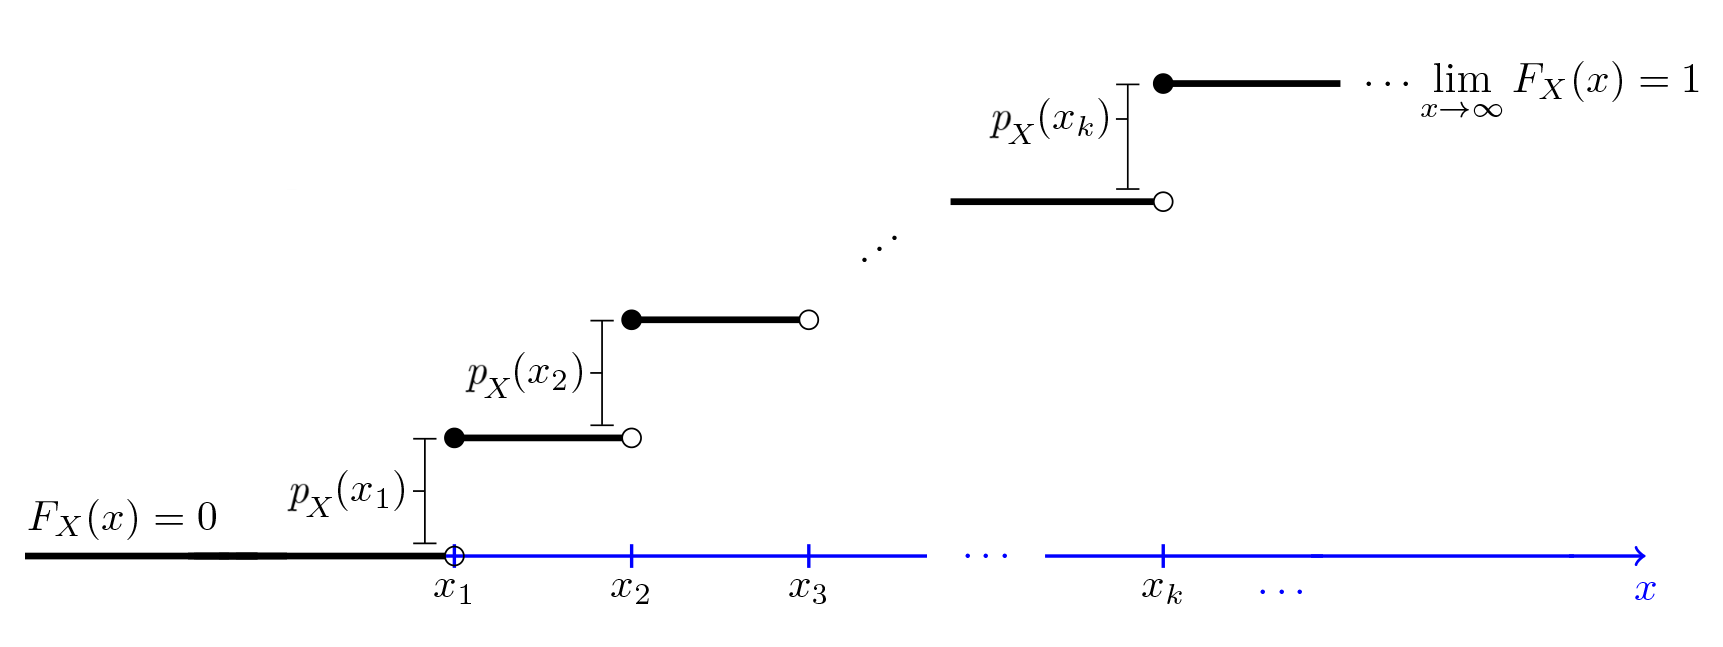
\includegraphics[width=0.8\linewidth]{chapters/chapter 9/CDF graph.png}
\end{figure}

որի խզումներին նայելիս կարելի է գլխի ընկնել, թե $X$-ը որ արժեքը ինչ հավանականությամբ \marginnote{$\PP[X=k]$-ն կգրենք $F_X(k) - F_X(k-1)$} է ընդունում։

{\rm PMF}-ը և {\rm CDF}-ը (որոնցից մեկը ունենալով՝ կարելի է ստանալ մյուսը) հարմար գործիքներ են տրված պատահական մեծության արժեքների վերաբերյալ պատկերացում կազմելու համար։ Պայմանավորվենք՝ այն, թե ի՞նչ արժեքներ է ընդունում պատահական մեծությունը, կամ որքա՞ն հավանականությամբ, կամ որքա՞ն է հավանական, որ այն մեծ/փոքր է այսինչ թվից, այդ ամենը անվանել պատահական մեծության \textit{բաշխում։}

Կասենք, որ գիտենք $X$-ի բաշխումը (կամ թե ինչպես են $X$-ի արժեքները բաշխված), եթե գիտենք նրա {\rm PMF}-ը կամ {\rm CDF}-ը։ Իսկ եթե ունենանք երկու պատահական մեծություններ, որոնք ունենան նույն բաշխումը, այսինքն՝ ցանկացած արժեք ընդունեն երկուսն էլ նույն հավանականությամբ, ապա կասենք, որ դրանք \textit{միատեսակ} են բաշխված:

\begin{definition}
$X$ և $Y$ պատահական մեծությունները կոչվում են \textbf{միատեսակ բաշխված,} \marginnote{անգլերեն՝ {\it identically distributed}} եթե նրանց {\it CDF}/{\it PMF}-ները համընկնում են։
\end{definition}

\warning{Միատեսակ բաշխված $\ne$ միմյանց հավասար։}

\begin{example}
Քննության է մտնում հաջորդ ուսանողը, որը ևս $15$ հարցից սովորել է $4$-ը։ Բնականաբար, հավանականությունը, որ նա կկտրվի կամ կանցնի քննությունը, նույնն է, ինչ առաջին ուսա\-նո\-ղի\-նը։ Հետևաբար եթե $X$-ով նշանակենք, թե քանի հարցի ճիշտ կպատասխանի առաջին ուսանողը, իսկ $Y$-ով՝ երկրորդը, ապա $p_X(k) = p_Y(k)$, և $X$-ն ու $Y$-ը կլինեն միատեսակ բաշխված։
\end{example}

Ասվածից, իհարկե, չի հետևում, որ երկու ուսանողն էլ պատասխանելու են նույն քանակով հարցերի․ $X$-ի ու $Y$-ի արժեքները կարող են իրարից տարբերվել,\marginnote{եթե չտարբերվեին, կլիներ նույն պատա\-հա\-կան մեծությունը՝ տարբեր տառե\-րով նշանակած} չնայած որ ցանկացած արժեք ընդունելու հավանականու\-թյունը երկուսի դեպքում էլ նույնն է։

\begin{example}
\\~
\begin{itemize}
\item Նետենք երկու զառ, $X$-ով նշանակենք առաջինի թիվը, $Y$-ով՝ երկրորդի։ Կրկին, $X$-ն ու $Y$-ը միատեսակ են բաշխված։ Դրա\-նով հանդերձ կարող են ընկնել ինչպես նույն թիվը, այնպես էլ տարբեր թվեր։%\marginnote{որքա՞ն է նույն թիվն ընկնելու հավանականությունը}

\item Նետենք մետաղադրամը և նշանակենք
\[
X = \begin{cases}
    1 & \text{եթե ընկնի գիր}\\
    0 & \text{եթե ընկնի ղուշ}
\end{cases}
\qquad 
Y = \begin{cases}
    0 & \text{եթե ընկնի գիր}\\
    1 & \text{եթե ընկնի ղուշ}
\end{cases}
\]
Այս դեպքում մետաղադրամը ինչ էլ ընկնի, $X$-ն ու $Y$-ը չեն կարող հավասար լինել։ Բայց դրանց բաշխումները համընկնում են, քանի որ
\[
\PP[X = 0] = \PP[X = 1] = \PP[Y = 0] = \PP[Y = 1] = 0.5
\]
\end{itemize}
\end{example}

\question{Ի՞նչ կասեք $X$-ի մասին, եթե $F_X$ ֆունկցիան բացասական կետերում $0$ է, դրականներում՝ $1$:}


\section{Անընդհատ պատահական մեծություններ}

Պատկերացնենք այսպիսի իրավիճակ։ Օդում թռչող ճանճը մոտենում է տետրում նկարված $[0, 10]$ հատվածին և պատահականորեն նստում որևէ կետում (ընդ որում կարևոր չէ՝ բոլոր կետերը նույն հավանականությունն ունեն, թե ասենք մեջտեղի կետերն ավելի հավանական են)։

\begin{center}
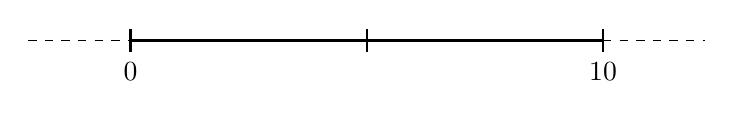
\begin{tikzpicture}
    \draw[dashed] (-1.3,0) -- (0,0);
    \draw[-, thick] (0,0) -- (6,0);
    \draw[dashed] (6,0) -- (7.3,0);
    
    \foreach \x in {0,3,6} {
    \draw[thick] (\x,0.15) -- (\x,-0.15);
    }
    
    \node[below, align=center] at (0,-0.15) {$0$};
    \node[below, align=center] at (6,-0.15) {$10$};
\end{tikzpicture}
\end{center}

Նշանակենք ճանճի նստած կետը $X$-ով և գտնենք դրա {\rm PMF}-ը։ 

\question{Որքա՞ն է հավանականությունը, որ $X = 5$։ Իսկ ասենք $\PP[X = 5.89]$-ը՞։}

Նախ, $X$-ի հնարավոր արժեքներն են $[0, 10]$ միջակայքի բոլոր կետերը․ $X$-ը դիսկրետ չէ։ Հետևաբար արժեքների քանակն այնքան մեծ է, որ առանձին վերցրած՝ ցանկացած կետի հավանականությունը $0$ է։ Ուրեմն 
\[
p_X(x) = 0
\]
բոլոր կետերում։ Հետևաբար $\PP[{X = \text{ինչ-որ թիվ}}]$ հարցնելը ոչ մի իմաստ չունի․ $p_X$ ֆունկցիան միշտ $0$ է և ունակ չէ որևէ բան ասել $X$-ի արժեքների մասին։

Ուրեմն հավանականային ֆունկցիան այս դեպքում չի աշխատում։ Փոխարենը օգնության է գալիս բաշխման ֆունկցիան, որն այս դեպքում ևս շարունակում է աշխատել․ եթե $\PP[X = 5]$-ը զրո է, ապա $\PP[X \le 5]$-ը միևնույն է՝ դրական թիվ է, որը ցույց է տալիս $5$ կետից ձախ նստած լինելու հավանականությունը՝
\[
F_X(5) = \PP[X \le 5] = \PP[X < 5]
\]
Հետևաբար {\rm CDF}-ից օգտվելով կարող ենք չափել $X$-ի արժեքի՝ ցանկացած $(a, b)$ միջակայքում գտնվելու հավանականությունը․
\[
\PP[X \in (a, b)] = \PP[a < X < b] = F_X(b) - F_X(a)
\]
իսկ $a$ և $b$ կետերի հավանականությունը կլինի $0$:

\begin{center}
\begin{tikzpicture}
    \draw[dashed] (-1.3,0) -- (0,0);
    \draw[-, thick] (0,0) -- (6,0);
    \draw[dashed] (6,0) -- (7.3,0);
    
    \fill[myblue!20] (1,-0.2) rectangle (2.5,0.2);
    
    \draw[thick, myblue] (1,0) -- (2.5,0);

    \filldraw[fill=white, draw=myred, thick] (4.5,0) circle (2pt);

    \foreach \x in {0,3,6} {
    \draw[thick] (\x,0.15) -- (\x,-0.15);
    }
    
    \node[below, align=center] at (0,-0.15) {$0$};
    \node[below, align=center] at (6,-0.15) {$10$};

    % \node[below=12pt, align=center] at (4.5,0) {
    %     \textcolor{myred}{\large $\bullet$} \hspace{0.4em} Important Point
    % };

    \node[below=12pt, align=center] at (1.75,0) {
        $\PP[$\tikz{\fill[myblue!20] (0,0) rectangle (1.8em,1.3ex);}$] > 0$
    };
    \node[below=12pt, align=center] at (4.5,0) {
        $\PP[$\tikz{\filldraw[fill=white, draw=myred, semithick] circle (1.75pt);}$] = 0$
    };
\end{tikzpicture}
\end{center}

Եթե մեզ ամեն դեպքում հետաքրքիր է եթե ոչ $X=5$ լինելու, ապա գոնե $5$-ին մոտիկ արժեքներ ընդունելու հավանականությունը, կարող ենք վերցնել ասենք՝ $5$ կետի կողքը մի փոքր միջակայք և հաշվել դրա հավանականությունը․
\[
\PP[X \in (5-h,\, 5+h)] = F_X(5+h) - F_X(5-h)
\]
\question{Կռահո՞ւմ եք, թե որ կողմ է խոսակցությունը գնում։}
Սա մեզ կտա $5$ արժեքին շատ մոտ լինելու հավանականությունը, իսկ որպեսզի հասկանանք՝ որքա՞ն է բուն $5$-ի ներդրումը, այսինքն՝ $5$ կետին մոտենալիս ինչքա՞ն է հավանականությունը \marginnote{եթե $5$-ը գանք անցնենք, բայց հավանա\-կա\-նու\-թյու\-նը չփոխվի, կստացվի, որ $5$-ը «կշիռ» չունի} մեծանում կամ փոքրանում, բաժանենք այս թիվը միջակայքի երկարության վրա՝
\[
\frac{F_X(5+h) - F_X(5-h)}{2h}
\]
և ձգտեցնենք $h$-ը զրոյի։ 

Ստացված թիվը կլինի $F_X$-ի ածանցյալը, որը կանվանենք $5$ կետում $X$-ի բաշխման \textit{խտություն։}

\begin{definition}
Եթե $X$-ը անընդհատ պատահական մեծություն է, իսկ $f_X(x)$-ն այնպիսի ֆունկցիա է, որ ցանկացած $c \in \R$ թվի համար
\[
F_X(c) = \int_{-\infty}^{c} f_X(t) \, dt 
\]
ապա $f_X$-ը կանվանենք $X$-ի \textbf{խտության ֆունկցիա} կամ {\aroff \textbf{\textit{PDF}:}}\marginnote{\it probability density function}}
\end{definition}

Այսինքն խտության ֆունկցիան բաշխման ֆունկցիայի ածանցյալն է՝\marginnote[*+2]{$F_X$-ը չնվազող է $\Rightarrow$ $f_X \ge 0$}
\[
F_X'(x) = f_X(x)
\]
Խոսքը, իհարկե, այն կետերի մասին է, որոնցում $F_X$-ն ունի ածանցյալ։

Իսկ սահմանման մեջ նշված բանաձևն ասում է, որ $\PP[X \le c]$-ն հաշվելու համար պետք է ինտեգրել այս $f_X$-ը մինչև $c$ թիվը, այսինքն $(-\infty, c)$-ում արժեք ընդունելու հավանականությունը հավասար է $(-\infty, c)$ միջակայքում $f_X$-ի գրաֆիկի տակ եղած \textit{մակերեսին։}

Խտության ֆունկցիան կարող է ընդունել տարբեր տեսքեր, ասենք՝ ճանճը կարող է նախապատվություն տալ $0$ կետին ավելի մոտ ար\-ժեք\-ներին կամ նախընտրել նստել մեջտեղում․

\begin{figure}[h]
    \centering
    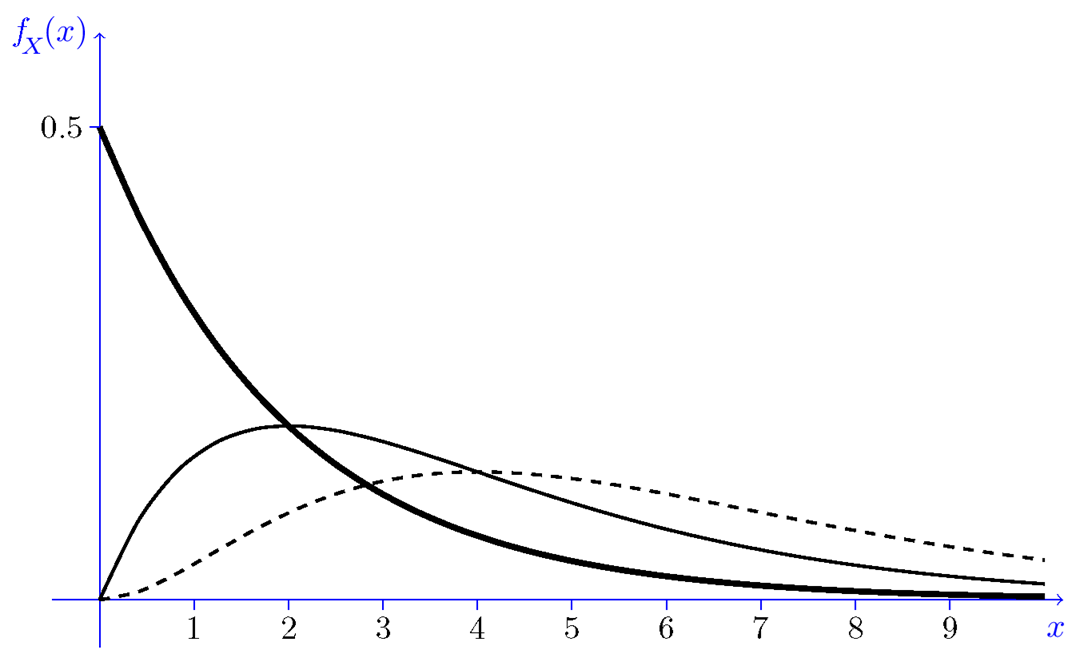
\includegraphics[width=0.8\linewidth]{chapters/chapter 9/PDF graph.png}
    \caption*{երեք տարբեր հնարավոր {\rm PDF}-ներ՝ կախված ճանճի ճաշակից}
\end{figure}

\question{{\it PDF}-ներից յուրաքանչյուրի դեպքում ո՞ր միջակայքում է ամենահավանական, որ ճանճը կնստի։}

Ինչպես դիսկրետ պատահական մեծության դեպքում {\rm PMF}-ին, այնպես էլ անընդհատ պատահական մեծության դեպքում՝ նրա {\rm PDF}-ին նայելով կարող ենք ստանալ բազմաթիվ տեղեկություններ նրա հնարավոր արժեքների ու դրանց հավանականությունների մասին։ 

Օրինակ՝ վերևի գրաֆիկներից յուրաքանչյուրում խտության ֆունկցիան $0$-ից ձախ և $10$-ից աջ զրո է, հետևաբար եթե չիմանայինք էլ՝ նայելով կհասկանայինք, որ $X$-ի հնարավոր արժեքները $[0, 10]$-ն են։ Կարող ենք նաև ասել, որ եթե $f_X$-ի արժեքը մեծ է օրինակ՝ $x=2$ կետում, ապա $X$-ը մեծ հավանականությամբ է արժեքներ ընդունում $2$ կետի հարևան շրջակայքում։ 

Ըստ էության՝ {\rm PDF}-ը {\rm PMF}-ի անալոգն ու փոխարինողն է անընդհատ պատահական մեծությունների համար։ Ինչպես դիսկրետ դեպքում $p_X$-ը, այնպես էլ անընդհատ դեպքում $f_X$-ը չի կարող լինել բացասական՝ 
\[
f_X(x) \ge 0 \qquad \text{ցանկացած $x\in\R$ կետում}
\]
սակայն քանի որ վերջինս հավանականություն չի ցույց տալիս (այլ ընդամենը դրա խտությունը), ապա $f_X$-ը կարող է ընդունել $1$-ից մեծ արժեքներ։ Վերջինիս սահմանումից նաև հետևում է, որ 
\[
\int_{-\infty}^{+\infty} f_X(t)\, dt = F_X(+\infty) = \PP[X \le +\infty] = 1 
\]
քանի որ․․․ ինչպե՞ս կարող է $X$-ը լինել $+\infty$-ից մեծ։

\question{Ունենալով $f_X$-ը՝ ինչպե՞ս գտնել $\PP[a < X < b]$-ն։}

Ամենահաճելի հատկությունը, որի շնորհիվ կարող ենք կիրառել խտության ֆունկցիան՝
\[
\PP[a < X < b] = \int_{a}^{b} f_X(t)\, dt
\]
այսինքն հավանականությունը, որ $X$-ն ընկած է $(a, b)$ միջակայքում հավասար է այդ միջակայքում նրա {\rm PDF}-ի տակ ընկած մակերեսին։

% Նշենք, որ երբեմն անընդհատ պատահական մեծությունները կարող են չունենալ խտություն, բայց 


\section{Հավասարաչափ բաշխում}

Փակենք մեր աչքերն ու մատը դնենք $[0, 10]$ հատվածում որևէ պա\-տա\-հա\-կան $X$ կետի վրա։
Կունենանք մի իրավիճակ, որը շատ նման է ճանճի դեպքին՝ այն տարբերությամբ, որ եթե ճանճը կարող է հակված լինել նստել ավելի ձախ կամ ավելի աջ գտնվող կետերում, և հատ\-վածի տարբեր մասերում նստելու հավանականությունը կարող է տարբեր լինել, ապա\marginnote{նույն երկարությամբ ցանկացած երկու միջակայք նույնչափ հավանական են՝
\[\PP[X \in (1.3, 1.5)] = \PP[X \in (4.7,4.9)]\]} այս օրինակում կարող ենք համարել, որ աչքերը փակ ընտրելիս որևէ նախապատվություն չկա․ ոչ մի թվի մոտ նշելու հավա\-նա\-կա\-նու\-թյունը մյուսից ավել չէ։ 

\question{Ըստ Ձեզ՝ ի՞նչ տեսք կունենա $X$-ի խտության գրաֆիկը։}

$[0, 10]$ հատվածի փոխարեն վերցնենք ավելի ընդհանուր՝ $[a, b]$ հատվածը, և երկրաչափորեն փորձենք պարզել $X$-ի բաշխումը։

Սկսենք {\rm CDF}-ից։ Քանի որ $X$-ի հնարավոր արժեքներն են $[a, b]$, ապա $a$-ից փոքր արժեք ընդունելու հավանականությունը $0$ է՝
\[
F_X(x) = \PP[X \le x] = 0 \qquad \text{եթե } x < a
\]
Պարզենք $F_X(x)$-ի արժեքը, երբ $a \le x \le b$։ 

\begin{center}
\begin{tikzpicture}
    \draw[dashed] (-1.3,0) -- (0,0);
    \draw[-, thick] (0,0) -- (6,0);
    \draw[dashed] (6,0) -- (7.3,0);    
    \draw[thick, myblue] (0,0) -- (4.5,0);
    \foreach \x in {6} {
    \draw[thick] (\x,0.15) -- (\x,-0.15);
    }
    \foreach \x in {0,4.5} {
    \draw[thick, myblue] (\x,0.15) -- (\x,-0.15);
    }
    \node[below, align=center] at (0,-0.15) {$a$};
    \node[below, align=center] at (6,-0.15) {$b$};
    \node[below, align=center] at (4.5,-0.15) {{\color{myblue} $x$}};
\end{tikzpicture}
\end{center}
Հավանականությունը, որ $X$-ը ընկած կլինի $[a, x]$ միջակայքում՝\marginnote{այստեղ արդեն կարող ենք օգտվել երկ\-րա\-չա\-փա\-կան հա\-վա\-նա\-կա\-նու\-թյունից}
\[
F_X(x) = \PP[X \le x] = \frac{\color{myblue} [a, x]\text{-ի երկարություն}}{[a, b]\text{-ի երկարություն}} = \frac{x-a}{b-a}
\]
Դե իսկ եթե $x$-ն ընկած լինի $b$-ից աջ,
\[
F_X(x) = \PP[X \le x] = \PP[X \le b] = 1
\]
և հետևաբար
\[
F_X(x) = \begin{cases}
    0 & \text{եթե } x < a\\
    \dfrac{x-a}{b-a} & \text{եթե } a \le x \le b\\
    1 & \text{եթե } x > b
\end{cases}
\]
Ստացանք $X$-ի բաշխման ֆունկցիան, և եթե այն \marginnote{$a$-ում ու $b$-ում $F_X$-ը ածանցյալ չունի, բայց դրանց կանտեսենք} ածանցենք՝
\[
f_X(x) = \begin{cases}
    \dfrac{1}{b-a} & \text{եթե } a \le x \le b\\
    0 & \text{մնացած կետերում}
\end{cases}
\]
կստանանք նաև $X$-ի խտության ֆունկցիան։

\begin{figure}[h]
    \centering
    \subfloat{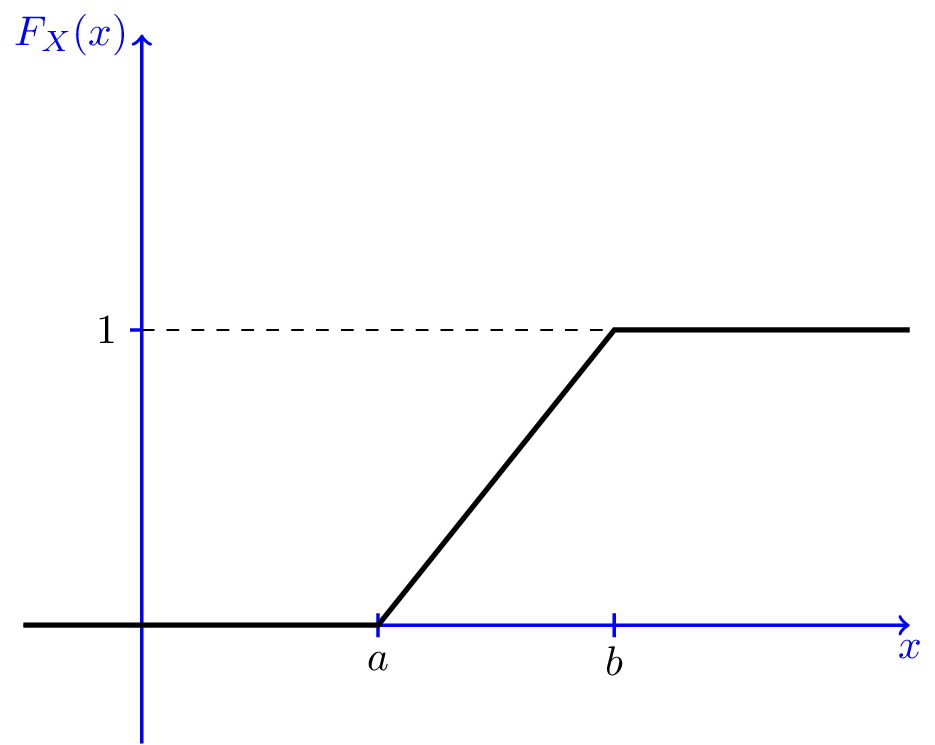
\includegraphics[width=0.4\linewidth]{chapters/chapter 9/uniform CDF.png}}%
    \qquad
    \subfloat{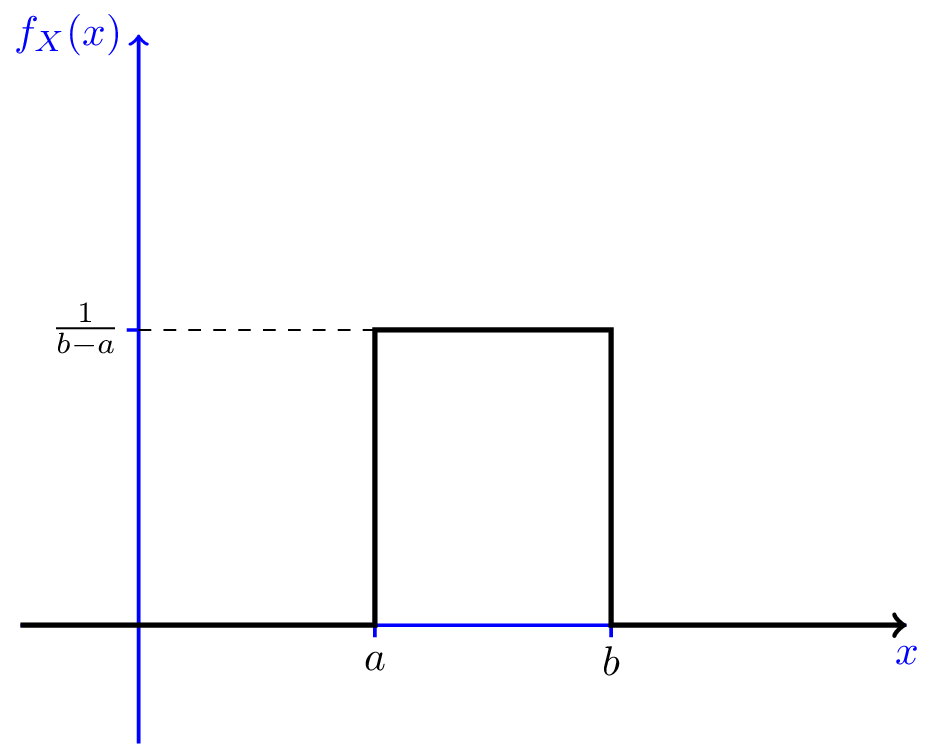
\includegraphics[width=0.4\linewidth]{chapters/chapter 9/uniform PDF.png}} %
\end{figure}

Նկատենք, որ $X$-ի {\rm PDF}-ն ունի մեր ակնկալած տեսքը՝ $[a, b]$-ից դուրս զրո է, իսկ ներսի բոլոր կետերում ընդունում է նույն արժեքը (ուրեմն ոչ մի կետի մոտ հավանականությունը մեծ կամ փոքր չէ), և նրա գրաֆիկի տակ եղած մակերեսը $1$ է։ Մյուս կողմից {\rm CDF}-ը $[a, b]$ միջակայքում գծորեն, այսինքն՝ հաստատուն արագությամբ աճում է։ 
Գրաֆիկների այս տեսքը մատնում է, որ գործ ունենք $[a, b]$-ում արժեքներ ընդունող և բոլորին հավասարապես վերաբերվող պատահական մեծության հետ (որին ժամանակն է անուն տալ)։

\begin{definition}
Կասենք, որ $X$ պատահական մեծությունը \textbf{հավասարաչափ} է բաշխված $(a, b)$ կամ $[a, b]$ \marginnote{անգլերեն՝ {\it uniformly distributed}}միջակայքում՝
\[
X \sim \operatorname{U}(a, b)
\]
եթե 
\[
f_X(x) = \begin{cases}
    \dfrac{1}{b-a} & \text{եթե } a \le x \le b\\
    0 & \text{մնացած կետերում}
\end{cases}
\]
\end{definition}


\section{Անկախություն}

Ենթադրենք նետել ենք երկու զառ։ Նախորդ թեմայում ասացինք, որ զառերի ելքերն իրար հետ կապ չունեն, հետևաբար դրանց հետ կապված ցանկացած երկու պատահույթ անկախ են՝ $\PP[A \cap B] = \PP[A] \cdot \PP[B]$: Մասնավորապես եթե $X$-ով նշենք առաջին զառի թիվը, իսկ $Y$-ով՝ երկրորդինը, ցանկացած $a$ ու $b$ թվերի համար կունենանք
\[
\PP[(X = a) \text{ և } (Y = b)] = \PP[X = a] \cdot \PP[Y = b]
\]
Նույն կերպ, եթե $X$-ով նշանակեինք առաջին զառի թվի քառակուսին, իսկ $Y$-ով ասենք՝ երկրորդի թվի մնացորդը $2$-ի բաժանելիս, միևնույն է դրանց համար այս երկու $\{X=a\}$ և $\{Y=b\}$ պատահույթները լինելու էին անկախ և դրանց \textit{համատեղ} {\rm PDF}-ը՝
\[
\PP[(X = a) \text{ և } (Y = b)]
\]
գրելու էինք արտադրյալով։ 
Տրամաբանական կլինի, եթե այս դեպքում նույնպես ասենք, որ $X$-ն ու $Y$-ը անկախ են։

\begin{definition}
$X$ և $Y$ դիսկրետ պատահական մեծությունները կոչվում են \textbf{անկախ,} եթե ցանկացած $a$, $b\in \R$ թվերի համար
\[
\PP[(X = a) \text{ և } (Y = b)] = \PP[X = a] \cdot \PP[Y = b]
\]
\end{definition}

Իհարկե, անընդհատ պատահական մեծությունների համար բոլոր այս երեք հավանականություններն էլ զրո են, հետևաբար ընդհանուր դեպքում անկախությունը կսահմանենք {\rm CDF}-ների միջոցով՝
\begin{definition}
$X$ և $Y$ պատահական մեծությունները կոչվում են\marginnote{և դիսկրետ, և անընդհատ դեպքում} \textbf{անկախ,} եթե ցանկացած $a$, $b\in \R$ թվերի համար
\[
\PP[(X \le a) \text{ և } (Y \le b)] = \PP[X \le a] \cdot \PP[Y \le b]
\]
\end{definition}

Մասնավորապես, եթե նետենք երկու զառ կամ մետաղադրամ (կամ ցանկացած նման պատահական փորձ կրկնենք երկու անգամ), և ստացվածները նշանակենք $X_1$-ով ու $X_2$-ով, դրանք կլինեն անկախ և միատեսակ բաշխված պատահական \marginnote{առաջին տառերով՝ {\rm i.i.d.}} մեծություններ։



\bigskip 

\begin{theory}
.
\begin{itemize}
\item կարդալ [{\rm Blitzstein-Hwang}], 91-94 (պատահական մեծու\-թյուն), 94-99 ({\rm PMF}), 108-109 ({\rm CDF}), 117-119 (անկախու\-թյուն), 195-197 ({\rm PDF}), 201-202 էջերը 
\item տեսնել պատահական մեծությունների տարբեր \href{https://dlsun.github.io/skis/continuous/random-variables.html}{օրինակներ}
\item դիտել {\aroff PMF, CDF, PDF}-ի մասին օգտակար \href{https://www.youtu.be/yRbfLlTmPE8
}{տեսանյութ}
\item ըստ ցանկության՝ նաև մեկ այլ \href{https://youtu.be/IaSGqQa5O-M}{տեսանյութ} {\rm 3b1b}-ից
\end{itemize}
\end{theory}

\newpage

\section{Խնդիրներ}

\begin{problem}
Երկու անգամ նետում ենք զառը և նշանակում
\begin{align*}
X &= 1\text{-ին զառի թիվը} \\
Y &= 2\text{-րդ զառի թիվը} \\
Z &= \text{այդ երկուսից մեծագույնը} = \max\{X, Y\} 
\end{align*}
Կարո՞ղ եք գտնել $Z$-ի {\rm PDF}-ն ու {\rm CDF}-ը։
\end{problem}

\begin{problem}
Անին պատրաստեց մի արտասովոր զառ ($1$-$6$ թվերով), որի
\begin{itemize}
    \item զույգ ընկնելու հավանականությունը նույնն է, ինչ կենտ ընկնելունը
    \item բոլոր զույգ թվերի հավանականությունները նույնն են
    \item $1$ ընկնելու հավանականությունը $0.5$ է
\end{itemize}
Ի՞նչ տեսք ունի զառի ընկած թվի {\rm PMF}-ը։
\end{problem}

\begin{problem}
$10$ սմ երկարությամբ փայտը երկու պատահական կետերից կտրելով՝ բաժանում են $3$ կտորի։ Որքա՞ն է հավանական, որ այդ երեք կտորներով կարելի է կառուցել եռանկյուն։

\hint{Առաջին երկու կտորները նշանակենք $X$ և $Y$-ով։ Որքա՞ն կլինի երրորդ կտորը։ Եռանկյան համար անհրաժեշտ է, որ կող\-մերից ցանկացած երկուսի գումարը մեծ լինի երրորդից։}
\end{problem}

\begin{problem}\marginnote[*+0.5]{\href{https://www.youtu.be/ccNSU_TsUnQ}{լուծում}}
$(0, 10)$ միջակայքից պատահականորեն վերցնում են երեք թիվ՝
\[
X,\ Y,\ Z \sim \operatorname{U}(0, 10)
\]
իրարից անկախ և հավասարաչափ բաշխված։

Որքա՞ն է հավանականությունը, որ ստացված երկարությամբ հատված\-ներով կարելի է կառուցել եռանկյուն։
\end{problem}

\begin{problem}
$X$ պատահական մեծության խտության ֆունկցիան է՝
\[
f_X(x) = \begin{cases}
    ax^5& \text{եթե }0\le x \le 3 \\
    0& \text{մնացած դեպքերում}
\end{cases}
\]
որտեղ $a$ հաստատունի արժեքն անհայտ է։ Կարո՞ղ եք գտնել $a$-ն։
\end{problem}

\begin{problem}
Համակարգիչը գեներացնում է պատահական թվեր, ընդ որում գեներացված $X$ թվի խտության ֆունկցիան է՝
\[
f_X(x) = \begin{cases}
    1 - |x-1|& \text{եթե }0\le x \le 2 \\
    0& \text{մնացած դեպքերում}
\end{cases}
\]
Գևորգը որոշում է գեներացնել պատահական թիվ և $1$-ից մեծ թվի դեպքում գնալ զբոսնելու, փոքր թվի դեպքում՝ քնելու, իսկ $1$ թվի դեպքում՝ դաս անելու։ Պարզեք, թե
\begin{enumerate}
\item ո՞րն է $X$-ի {\rm CDF}-ը
\item որքա՞ն է հավանական, որ Գևորգը կգնա զբոսնելու
\item որքա՞ն է հավանական, որ Գևորգը դաս չի անի
\end{enumerate}
\end{problem}

\begin{problem}
Վերոնշյալ մարտավարության արդյունքում հավտեսի \marginnote[*-0.5]{\textit{հավ}անականությունների \textit{տես}ության} քննությանը Գևորգի պատասխանած հարցերի տոկոսը ցույց տվող $X$ պատահական մեծության բաշխման ֆունկցիան է՝
\[
F_X(x) = \begin{cases}
    0& \text{եթե } x < 0 \\
    \sqrt{x}& \text{եթե } 0 \le x \le 1 \\
    1& \text{եթե } x > 1
\end{cases}
\]
Որքա՞ն է հավանականությունը, որ Գևորգը ճիշտ կպատասխանի հար\-ցերի գոնե կեսին։  
\end{problem}